\subsection{Algunos ejemplos}

El objetivo de esta sección es brindar ejemplos concretos, con distintos datos de entrada, para mejorar el entendimiento de la funcionalidad de los mismos. El ruggedness o escarpamiento del terreno, por ejemplo, es algo que en principio cuesta entender pero que al comparar imágenes específicas se comprende mejor el funcionamiento.

El siguiente terreno fue generado con 300 divisiones (se ven menos en la imágen). 200 picos. de alturas entre 1 y 10, con un escarpado de 1.\footnote{Si se quiere generar, la semilla usada fue: 123456.} 

\begin{center}
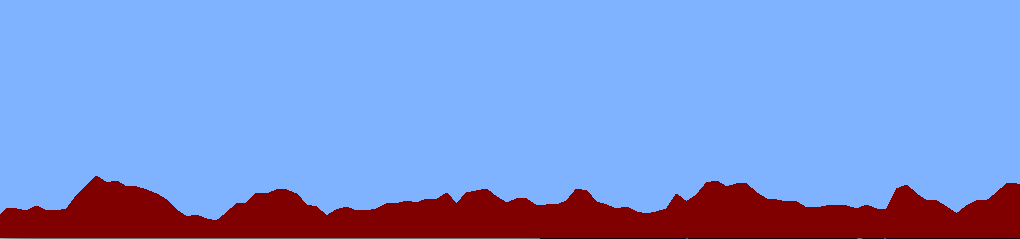
\includegraphics[scale=0.4]{imagenes/300-200-1-10-1-123456.png} 
\end{center}

A continuación utilizamos la misma entrada salvo por el escarpado, el cuál es de 10.

\begin{center}
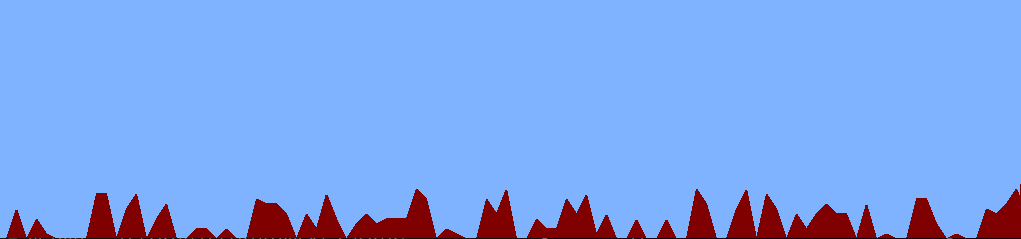
\includegraphics[scale=0.4]{imagenes/300-200-1-10-10-123456.png} 
\end{center}

Se puede ver cómo, al aumentar el escarpado, el terreno queda más abrupto. Esto se debe a que la influencia de los picos desciende con mayor velocidad, es decir, el rango de posiciones sobre las cuáles influye (y también el tamaño de su influencia) va decreciendo a medida que se aumenta el escarpado. Así, hay posiciones sobre las que antes influía que ahora no, o en menor medida, generando picos más aislados o separados.

\begin{center}
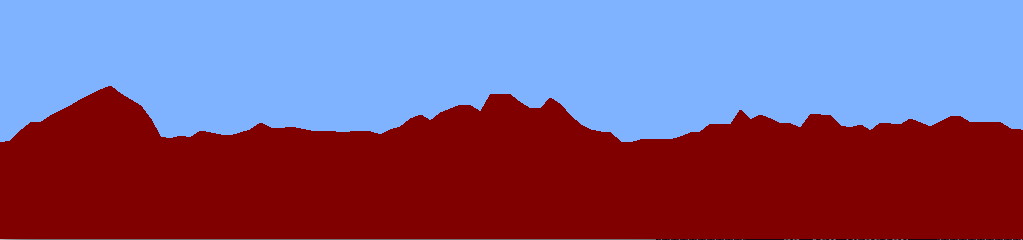
\includegraphics[scale=0.4]{imagenes/300-200-10-30-1-123456.png} 
\end{center}
En este caso variamos las alturas de los picos, ahora entre 10 y 30, utilizando la misma semilla y escarpado de 1. Como se puede observar, aumentar el tamaño de los picos no es mover la imágen más arriba, esto se debe a que las alturas se eligen al azar dentro de las posibles.

\begin{center}

\includegraphics[scale=0.4]{imagenes/300-10-1-10-1-123456.png} 
\end{center}
Por último queríamos mostrar qué sucede cuando hay muy poca proporción de picos. Éstos quedan aislados casi siempre y se genera un terreno que poco tiene que ver con la realidad, de todas maneras puede tener su utilidad, quizás en algún videojuego por ejemplo.